\chapter{Implementation and Protocol}


In this chapter, we translate the Spectrum by quantum walk algorithm from theory to a physically realizable implementation, by first providing a protocol with relevant quantum circuits. Then we show an implementation in \textit{ProjectQ} for the quantum chemistry problem of two systems, the element $H$ and the molecule $H_2$. Note that there is a distinct difference between these two: while they both carry the name hydrogen, $H_2$ is referred to as \textit{molecular} hydrogen while $H$ is the \textit{molecule} hydrogen.

\section{Protocol}

Throughout the description of the protocol of the algorithm, we consider the specifics of simulating the Hamiltoniam \todo{reference hamiltonian} of the hydrogen molecule. The first step is to assign the necessary quantum registers in the quantum computer. There are in total three registers: the \verb|physical| register, the \verb|ancillary| register and the \verb|counting| register. The \verb|physical| register is of size $n$, where $n$ is the number of qubits that the Hamiltonian acts on. The \verb|ancillary| register is of size $\log(N+1)$, the ceiling of the number of qubits required to describe $N$ terms, where $N$ is the number of terms in the Hamiltonian. The \verb|counting| register is the auxilliary register of the phase estimation procedure of $W$. The size of the register, denoted as $t$, depends on the desired success rate and accuracy of the phase estimation.\\

Next, the registers are to be initialized. We initialize the \verb|counting| register to $\ket{0}^{\otimes t}$ and subsequently apply $H^{\otimes t}$. We aim to prepare the rest of the system in the state

$$
B \ket{0} \otimes \tilde{\ket{\phi_0}}
$$

The $B$ operator maps the $\ket{0}$-state to $
=\sum_{j} \beta_{j}|j\rangle
$, so $B$ can be represented as an $N$-dimensional matrix where the leftmost column is filled with the coefficients of the rescaled Hamiltonian. This matrix is not unitary yet but as the rest of the matrix is not constrained, the matrix can be made unitary by the Gram-Schmidt process. There exists a myriad of methods for decomposing this matrix into single-qubit and CNOT gates. In our implementation, a pre-existing state-preparation function is used, which is an implementation of the general state preparation circuit introduced by \textcite{trans}. This method uses a sequence of uniformly controlled rotations with an upper bound for the complexity of \(2^{n+2}-4 n-4\) CNOT gates and \(2^{n+2}-5\) one-qubit operations.\\

The \verb|physical| register is to be prepared in $\ket{\tilde{\phi_0}}$, which has a large overlap with the actual ground state $\ket{\phi_0}$. We dicussed in more detail how to obtain such approximation for highly complex systems in \ref{subsec: zeno}. In our implementation of the hydrogen systems, eigenstates can be obtained by diagonalization as the Hamiltonian matrices are not computationally complex. We can artificially create an approximation of the ground state by mapping a superposition of the ground state and some excited states to the physical register. After the qubits are initialized, we need to define the subroutines that compose $W$. Let us first remind ourselves of the definition of the reflection operator $S$:

$$ S = B^{\dagger}\left(I - 2\ket{0} \bra{0} \right) B$$

$\left(I - 2 \ket{0} \bra{0} \right)$ maps $\ket{0}^{\otimes n}$ to $ - \ket{0}^{\otimes n}$ and acts as identity on all the other state, reminiscent of an inversely acting N-Controlled-Z operation. We can achieve this subroutine by first applying NOT to the entire register, then performing a N-Controlled-Z operation and ultimately re-applying NOT to the register. A circuit schematic of this subroutine is shown below.


\begin{figure}[h]
  \[
 \Qcircuit @C=1em @R=.7em {
    \lstick{a_0} & \multigate{3}{I-2\ketbra{0}{0}} & \qw \\
    \lstick{a_1} & \ghost{I-2\ketbra{0}{0}} & \qw \\
    \lstick{a_2} & \ghost{I-2\ketbra{0}{0}} & \qw \\
    \lstick{a_3} & \ghost{I-2\ketbra{0}{0}} & \qw
 }
 \quad \raisebox{-2.4em}= \quad
 \Qcircuit @C=1em @R=.7em {
    & \targ & \ctrl{1} & \targ & \qw \\
    & \targ & \ctrl{1} & \targ & \qw \\
    & \targ & \ctrl{1} & \targ & \qw \\
    & \targ & \gate{Z} & \targ & \qw \gategroup{1}{3}{4}{3}{.7em}{--}\\
    & & & & \\
    & & \mbox{$I - 2\ketbra{0}{0}$} & &
 }
\]
  \caption{Schematic of the subroutine $ \left(I - 2 \ket{0} \bra{0} \right)$ for $n = 4$.}
\end{figure}

This operation is enclosed between $B^{\dagger}$ and $B$. Moving onto $V$, this operation applies the $j$-th multi-qubit Pauli operator to the \verb|physical| register, controlled by the \verb|ancillary| register. This means that  To do so, we introduce another convention, namely a not gate applied to the target bit, conditional on the control bit being set to zero \cite{nielsen}. This effect is achieved by \\  \begin{equation} \label{xcx} X_{\text{control}} CNOT_{\text{control, target}} X_{\text{control}} \ket{\psi}\end{equation}.

\begin{figure}[h]
\[
    % somehow these circuits are normally not the same size so I made the left one bigger
    \Qcircuit @C=1em @R=1.2em {
        & \ctrlo{1} & \qw \\
        & \targ & \qw
    }
    \quad \raisebox{-.9em}= \quad
    \Qcircuit @C=1em @R=.7em {
        & \gate{X} & \ctrl{1} & \gate{X} & \qw \\
        & \qw & \targ & \qw & \qw
    }
\]
  \caption{Circuit schematic of the alternate controlled NOT operation, dependent on the control qubit being one.}
\end{figure}

This operation allows us to construct a circuit where an operation is applied, conditional on a register being set to a specific bit-string state. For example, the $V$ operation for $j = 5, \ket{5} = \ket{101}$: $\ket{5}\bra{5} \otimes P_5$ will only apply $P_5$ on the \verb|physical| register if the first ancillary qubit is 1, the second qubit 0 and the third qubit 1.

The circuit of the unitary walk operator $W$ is constructed by the successive application of the circuits of $S$ and $V$. Next, we perform phase estimation, whose circuit schematic can be shown in section 3.2. To recap, phase estimation consists of a series of controlled operations $W$, where for each qubit in the prepared \verb|counting| register, $W$ is applied to the \verb|physical| and \verb|ancillary| register $2^{t-1}$ times. This projects the phase of $W$ onto the \verb|counting| register, where the phase can be mapped directly to the \verb|counting| register by applying the inverse Fourier transform. Performing a measurement on the \verb|counting| register then reveals $E_k$.

\section{Implementation in ProjectQ}

This algorithm has been implemented for a general Hamiltonian in the open-source Python software framework for quantum computing by \textcite{steiger}. We've adapted the code for two Hamiltonians, the molecule hydrogen and molecular hydrogen. The full Jordan-Wigner reduced Hamiltonian for the molecule can be found in \ref{ham}, and the Hamiltonian for molecular hydrogen $H_2$ is

\begin{equation}
H=g_{0} \mathbb{1}+g_{1} Z_{0}+g_{2} Z_{1}+g_{3} Z_{0} Z_{1}+g_{4} Y_{0} Y_{1}+g_{5} X_{0} X_{1},
\end{equation} where the coefficients $g$ are functions of the hydrogen-hydrogen bond angle \cite{malley}. Both these Hamiltonians are simple enough for a classical computer to easily calulate its eigenstates and eigenvalues by diagonalization. For complex structures, an approximation of the groundstate has to be found via the method explained in \ref{subsec: zeno} or via Monte Carlo simulation \cite{poulin}. However, as we have access to the eigenstates classically, we can artificially create an approximation of the ground by creating a superposition of the ground state and an excited state. But before we cover the results of the Hamiltonian simulation, let us illustrate the implementation by taking a trivial Hamiltonian and reducing all the register sizes to one. The following circuit is a drawing of all the operations with the simplified parameters, generated by the python package Matplotlib via ProjectQ.

\begin{figure}[h]
  \center 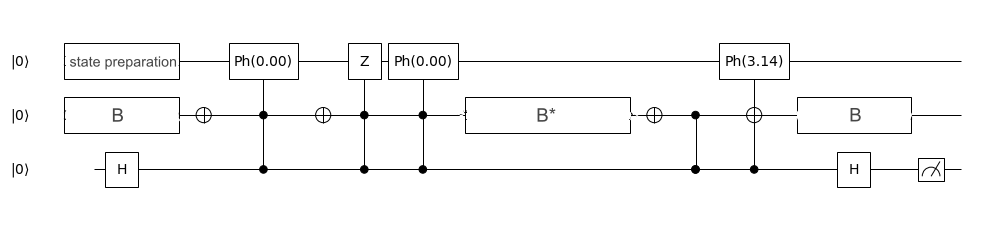
\includegraphics[width = \textwidth]{circuit.png}
  \caption{Circuit of the Spectrum by quantum walk implemented in ProjectQ, for single-qubit registers and trivial Hamiltonian.}
\end{figure}

The first register is the \verb|physical| register, the second register is the \verb|ancillary| register and the final register is the \verb|counting| register. While there is some non-conventional, ProjectQ-specific notation in the Pauli operations, this drawing shows that the implementation follows the protocol discussed above.

\section{Results}
Before we show the results of the implementation, let us motivate the state preparation sequence used. As we can obtain the ground state corresponding to the specific Hamiltonian classically, we artificially create an approximation of the ground state by preparing a superposition of the classicaly obtained eigenstates. We first show that the distribution of obtained energies is directly related to the probabilites of the states in the superposition of the approximated ground state. After we have shown this relation, we then try to get energy measurements of $H_2$ and $H$ as accurately as possible by treating the best case scenario, in which the \verb|physical| register is prepared in the classically obtained ground state. We acknowledge that this is not conform protocol for more complex systems of which we cannot just obtain the eigenstates classically. In section \ref{subsec: zeno} we show how to prepare an approximation of the ground state in such case. However, the added inaccuracy of non-ground energy measurements we'd introduce is rather trivial, as we can predict the energy distribution anyway. With our precise energy measurements, we aim to show that this algorithm, when the input is the ground state, returns energies that match the exact, well-established values with a certain accuracy.

\vspace{5mm}
First we consider the results of energy measurements on an approximation of the groundstate. We prepare the physical register in an equal superposition of the actual ground state and some excited state:
\begin{equation}
  \ket{\tilde{\phi}} = \frac{1}{\sqrt{2}} \ket{\phi_0} + \frac{1}{\sqrt{2}} \ket{\phi_k}
\end{equation} Perfoming a series of iterations of the algorithm result in the energy distribution plotted in \ref{distr}.

\begin{figure}[h] \label{distr}
  \center 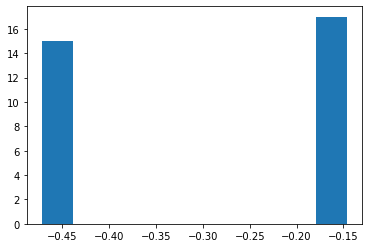
\includegraphics[width = 0.5\textwidth]{proofofsuper.png}
  \caption{Energy distribution of 32 iterations of the algorithm with a phase estimation precision of $t = 8$.}
\end{figure}

As the distribution of energies is directly related to the probability of the corresponding basis state in the approximation, this result matches our expectation, given the probabilities of $\frac{1}{2}$. The energy corresponding to the second peak is roughly 0.15 Hartree. This matches the first excited state of the hydrogen atom The ground energy seems close to the theoretical value and we now perform a series of highly precise measurements on the ground state, of which the result is displayed below.

\begin{figure}[h]
  \center 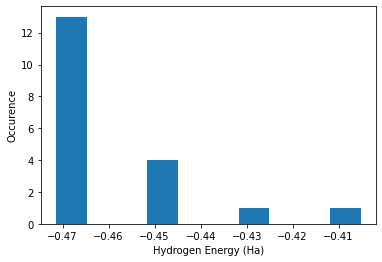
\includegraphics[width = 0.5\textwidth]{ground.png}
  \caption{A sampling of energy measurements when the physical register is prepared in the ground state.}
\end{figure}

The small fluctuations seen are due to the present imprecision in the phase-estimation process. The lowest energy sampled is $-0.4714$ Hartree, with a phase estimation accuracy of $t = 10$. The theoretical value of the ground energy of the hydrogen molecule is $-0.5$ Hartree. As the Jordan-Wigner mapping is exact and the Born-Oppenheimer approximation is considered in the theoretical value, this inaccuracy is caused by a combination of the limited accuracy of phase estimation and inaccuracies of the state preparation.\\

Next, we implement the $H_2$ molecule's Hamiltonian, where each sequence we find the ground energy corresponding to the bond length in Angstrong. We've performed three different sequences of measurements with a respective phase estimation accuracy of $t=8$, $t = 9$, $t=10$. The results are plotted below.

\begin{figure}
    \centering
    \begin{subfigure}[b]{0.48\textwidth}
        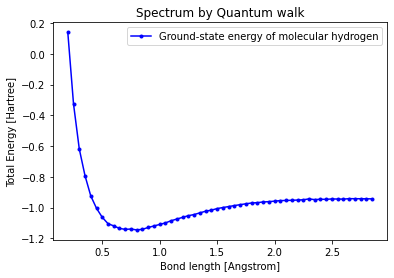
\includegraphics[width= \textwidth]{h2_10.png}
        \caption{Potential energy of $H_2$ against bond angle, calculated by the spectrum by quantum walk algorithm for a phase estimation precision of $t= 10$}
        \label{fig:mouse}
    \end{subfigure}

    \begin{subfigure}[b]{0.48\textwidth}
        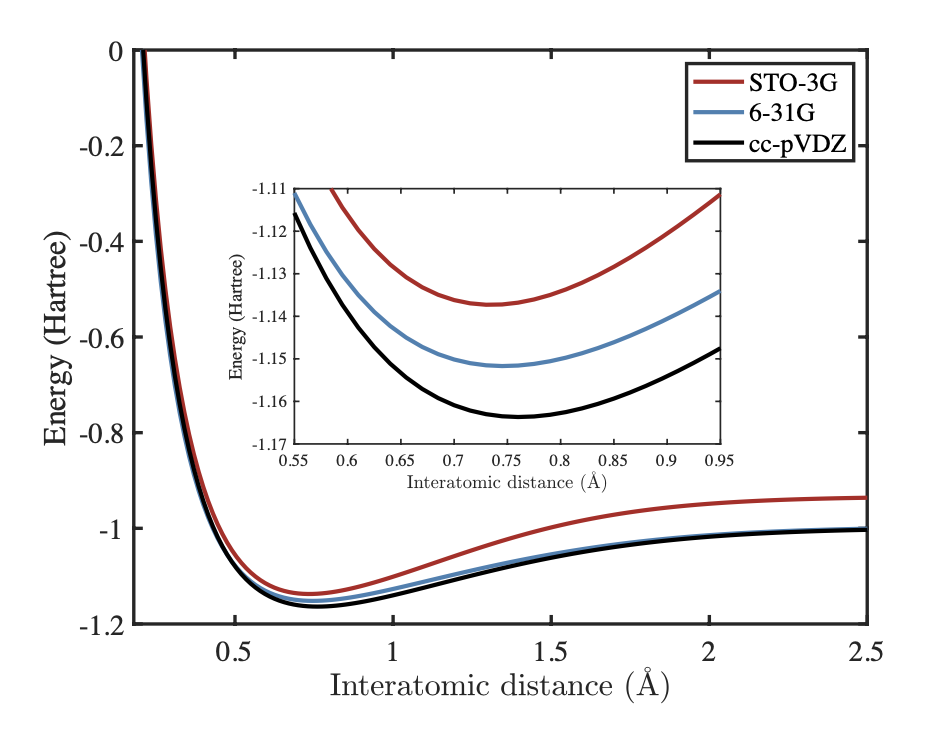
\includegraphics[width= \textwidth]{h2curv.png}
        \caption{Exact potential curves of $H_2$ for different basis sets \cite[p.~42]{McArdle}}
        \label{fig:tiger}
    \end{subfigure}
    ~ %add desired spacing between images, e. g. ~, \quad, \qquad, \hfill etc.
    %(or a blank line to force the subfigure onto a new line)
    % \caption{The ground energy of $H_2$, plotted against the bond length in Angstrong for three different precisions of $t$}\label{fig:animals}
\end{figure}

\newpage

\chapter{Discussion and Conclusion}


The main drawback of the Spectrum by quantum walk algorithm is that before implementing $W$, we have to rescale the coefficients of the Hamiltonian by a factor of $\mathcal{N}$. By doing so, we rescale the spectrum as the spectral gap (the difference between the ground state and the first excited state) with that same factor \cite{steiger, poulin}. This is problematic as the resolution of the energy measured is lowered by the rescaling. When compared to Trotterization, which implements an approximation of the time evolution operator $\exp{-iHt}$, $W$ needs to be applied $\mathcal{N} t$ times to achieve the level of accuracy obtained by Trotterization \cite[p.~87]{steiger}. Whether implementing $W$ is more efficient than Trotterization depends on the Hamiltonian in question as well as the number of Trotter steps needed to implement the time-evolution operator. Ultimately we aim to simulate large molecules and as we currently do not have the resources to simulate complex Hamiltonians, we are unable to estimate the advantage of the Spectrum by quantum walk algorithm.
